\documentclass[11pt]{tg_usta}
% Informe TALLER-2 — Construcción de Ontología y Análisis Semántico con WordNet
% Basado en la plantilla LaTeX del TALLER-1 (tg_usta.cls, PUJ)
\usepackage{tcolorbox}
\usepackage{float}
\usepackage{graphicx}
\usepackage{makecell}
\usepackage{anysize}
\usepackage{cite} % para contraer referencias
\marginsize{1in}{1in}{1in}{1in} %% Márgenes NO MODIFICAR
% Cargar los paquetes necesarios aquí
\usepackage{amsmath,amsthm,amssymb}
\usepackage{multicol}
\usepackage{url}
\usepackage{multirow}
\usepackage{tikz}
\usepackage[T1]{fontenc}
\usepackage{array}
\usepackage{booktabs}
\usetikzlibrary{trees}
% babel: la clase tg_usta ya carga [spanish]; se mantiene el nombre 'Tabla'
\renewcommand{\tablename}{Tabla}
\usepackage[utf8]{inputenc}
\usepackage{graphicx}
\usepackage{subcaption}
\usepackage{listings}

\newtheorem{definicion}{Definición}[section]
\newtheorem{nota}{Nota}[section]
\newtheorem{problema}{Problema}[section]
\newtheorem{teorema}{Teorema}[section]
\newtheorem{corolario}{Corolario}[section]
\newtheorem{proposicion}{Proposición}[section]
\newtheorem{lema}{Lema}[section]
\allowdisplaybreaks
\decimalpoint

\begin{document}
\title[maintitle = Construcción de Ontología y Análisis Semántico con WordNet.,
       secondtitle = Taller 2 - Procesamiento de Lenguaje Natural]

\begin{authors}[Rivera, Carrillo, Garnica \& Prieto]

\author[affiliation = PUJ,
        firstname = Erika Valeria,
        surname = Rivera Jimenez,
        email = riveraev@javeriana.edu.co]

\author[affiliation = PUJ,
        firstname = Julian Guillermo,
        surname = Carrillo Meneses,
        email = carrillojuliang@javeriana.edu.co]

\author[affiliation = PUJ,
        firstname = Carlos Andres,
        surname = Garnica Salazar,
        email = carlos\_garnicas@javeriana.edu.co]

\author[affiliation = PUJ,
        firstname = Oscar Andres,
        surname = Prieto Moreno,
        email = o-prieto@javeriana.edu.co]

\end{authors}

\begin{mainabstract}

El presente informe técnico describe la construcción de una ontología OWL a partir del Tesauro de la Comisión de la Verdad (CEV), el enriquecimiento léxico de sus conceptos mediante WordNet (NLTK y Open Multilingual WordNet) y su explotación formal con consultas SPARQL. Se seleccionaron seis grupos de tesauros (609 términos) con criterios cuantitativos que cubren el ciclo del conflicto armado colombiano: actores, hechos victimizantes, armas, poblaciones, impactos y afrontamientos. La ontología resultante (623 clases, 534 individuos, 17 propiedades de objeto y 6 clases definidas con restricciones) es consistente según el razonador HermiT y fue validada en Protégé. El análisis con WordNet en español alcanzó una cobertura del 50,5\,\% sobre 610 conceptos (54.130 relaciones de los nueve tipos semánticos), y se ejecutaron 22 consultas SPARQL documentadas, incluidas las que recorren el ciclo causal completo del conflicto. El informe responde, como eje central, a la pregunta del taller sobre las ventajas de representar conocimiento en ontologías frente a un análisis plano de texto en PLN: semántica explícita y compartida, razonamiento e inferencia automática, reutilización interoperable y complementariedad con las técnicas estadísticas. \\\\
 \textit{\textbf{Palabras clave:}} Ontologías, WordNet, Tesauro, OWL, SPARQL, Comisión de la Verdad, Procesamiento de Lenguaje Natural
 \end{mainabstract}


\section{Introducción}

El esclarecimiento de los patrones y causas del conflicto armado colombiano exigió a la Comisión para el Esclarecimiento de la Verdad (CEV) la normalización de una cantidad masiva de información documental. Su Tesauro (2022) reúne más de 12.000 términos organizados en núcleos, dominios y directorios, con relaciones de jerarquía (TG/TE), equivalencia (USE/UP) y asociación (TR). Este taller parte de ese recurso para construir una ontología formal: un artefacto OWL en el que las entidades, las jerarquías y las relaciones del dominio quedan representadas de forma explícita, razonable y consultable.

El trabajo comprende cuatro hitos: (i) la selección y justificación de cinco grupos de tesauros ampliados a seis con el grupo de afrontamientos y resistencias no violentas, completando el ciclo del conflicto; (ii) la construcción de la ontología en formato OWL con un modelo semántico fuerte (17 propiedades de objeto con pares inversos, 7 axiomas del ciclo y 6 clases definidas); (iii) la implementación en Python de un motor que extrae las nueve relaciones semánticas de WordNet sobre los conceptos de la ontología; y (iv) la formulación y ejecución de consultas SPARQL documentadas.

Más allá de los resultados numéricos, el taller plantea una pregunta de fondo que estructura este informe: \textit{¿qué ventajas aporta representar conocimiento en ontologías frente a un análisis plano de texto en PLN?} La respuesta se desarrolla en la sección de reflexión, apoyada en la evidencia empírica de este trabajo: inferencias que el razonador deriva sin estar escritas, consultas causales que ningún pipeline estadístico puede garantizar y un artefacto interoperable y reutilizable.


\section{Datos y metodología}

\subsection{Fuente de datos: Tesauro CEV 2022}

La fuente es el Excel del Tesauro CEV 2022, con la hoja ``Tesauro'' de \textbf{12.341 términos} en \textbf{41 grupos} (núcleos, dominios y directorios). La jerarquía está codificada en el propio término con el separador `` - '' y alcanza entre 1 y 10 niveles de profundidad, con el 74\,\% de los términos entre los niveles 3 y 5. El control de calidad es alto: solo 3 duplicados en todo el archivo.

\subsection{Selección de los seis grupos}

Sobre los 41 grupos se aplicaron cinco criterios cuantitativos: (i) tamaño entre 50 y 450 términos; (ii) profundidad jerárquica representativa; (iii) cobertura de WordNet en español $\geq 1$\,\% (sondeo previo con omw-1.4); (iv) relevancia temática para el mandato de la CEV; y (v) diversidad de ejes semánticos. A los cinco grupos resultantes se sumó un sexto ---\textit{Afrontamientos y resistencias no violentas - cotidianas}--- para completar el ciclo del conflicto \textbf{Actor $\rightarrow$ Hecho $\rightarrow$ Población $\rightarrow$ Impacto $\rightarrow$ Afrontamiento}. La Tabla \ref{tab:grupos} resume los seis grupos seleccionados, que suman \textbf{609 términos}.

\begin{table}[H]
    \centering
    \caption{Grupos del Tesauro CEV seleccionados para la ontología.}
    \small
    \setlength{\tabcolsep}{4pt}
    \begin{tabular}{l r r}
    \hline
    Grupo & Términos & Cobertura WordNet-es \\
    \hline
    Actores armados y otros participantes en las dinámicas de la guerra & 82 & 14,6\,\% \\
    Impactos & 107 & 11,2\,\% \\
    Armas & 94 & 7,5\,\% \\
    Poblaciones & 213 & 1,4\,\% \\
    Hechos victimizantes & 90 & 2,2\,\% \\
    Afrontamientos y resistencias no violentas - cotidianas & 23 & 4,3\,\% (exacta) \\
    \hline
    \textbf{Total} & \textbf{609} & --- \\
    \hline
    \end{tabular}
    \label{tab:grupos}
\end{table}

\subsection{Construcción de la ontología OWL y modelo semántico}

La ontología se construyó con \texttt{owlready2} y se serializó en RDF/XML bajo el IRI \texttt{http://www.semanticweb.org/cev/tesauro\#}. A partir de los 609 términos se derivaron \textbf{623 clases}: 610 conceptos del tesauro (incluidos los nodos sintéticos que completan la jerarquía), 6 clases definidas y la superclase \texttt{ConceptoDelTesauro}. Los \textbf{534 términos hoja} se modelaron además como individuos. Las \textbf{17 object properties} se organizan en dos familias:

\begin{itemize}
    \item \textbf{Estructurales:} \texttt{esParteDe}/\texttt{parteDe} (meronimia del tesauro), \texttt{relacionadoCon} (simétrica, 50 axiomas TR) y \texttt{perpetradoPor}/\texttt{esVictimaDe} (12 axiomas hecho-actor).
    \item \textbf{Modelo semántico del ciclo del conflicto} (6 pares inversos): \texttt{afectaA}/\texttt{esAfectadaPor}, \texttt{generaImpacto}/\texttt{esGeneradoPor}, \texttt{experimentaImpacto}/\texttt{impactaA}, \texttt{desarrollaAfrontamiento}/\texttt{esDesarrolladoPor}, \texttt{respondeA}/\texttt{esRespondidoMediante} y \texttt{empleaArma}/\texttt{esEmpleadaEn}, con 7 axiomas raíz que cierran el ciclo a nivel de clase.
\end{itemize}

Además se definieron \textbf{6 clases definidas} con restricciones (\texttt{owl:equivalentClass}), que el razonador clasifica automáticamente: \texttt{HechoPerpetradoPorActor} $\equiv$ Hechos $\cap$ \texttt{perpetradoPor} SOME Actores; \texttt{PoblacionAfectadaPorHechos} $\equiv$ Poblaciones $\cap$ \texttt{esAfectadaPor} SOME Hechos; \texttt{PoblacionConImpacto}; \texttt{PoblacionConAfrontamiento}; \texttt{HechoQueGeneraImpacto} y \texttt{AfrontamientoAsociadoAHecho}. El grafo resultante contiene \textbf{9.812 triples}; la validación fue triple: parseo con rdflib, consistencia con el razonador \textbf{HermiT} ---que además clasifica: \texttt{DesplazamientoForzado} es inferido subclase de \texttt{HechoPerpetradoPorActor}--- y apertura sin errores en \textbf{Protégé 5.6.9}.

\begin{figure}[htbp]
    \centering
    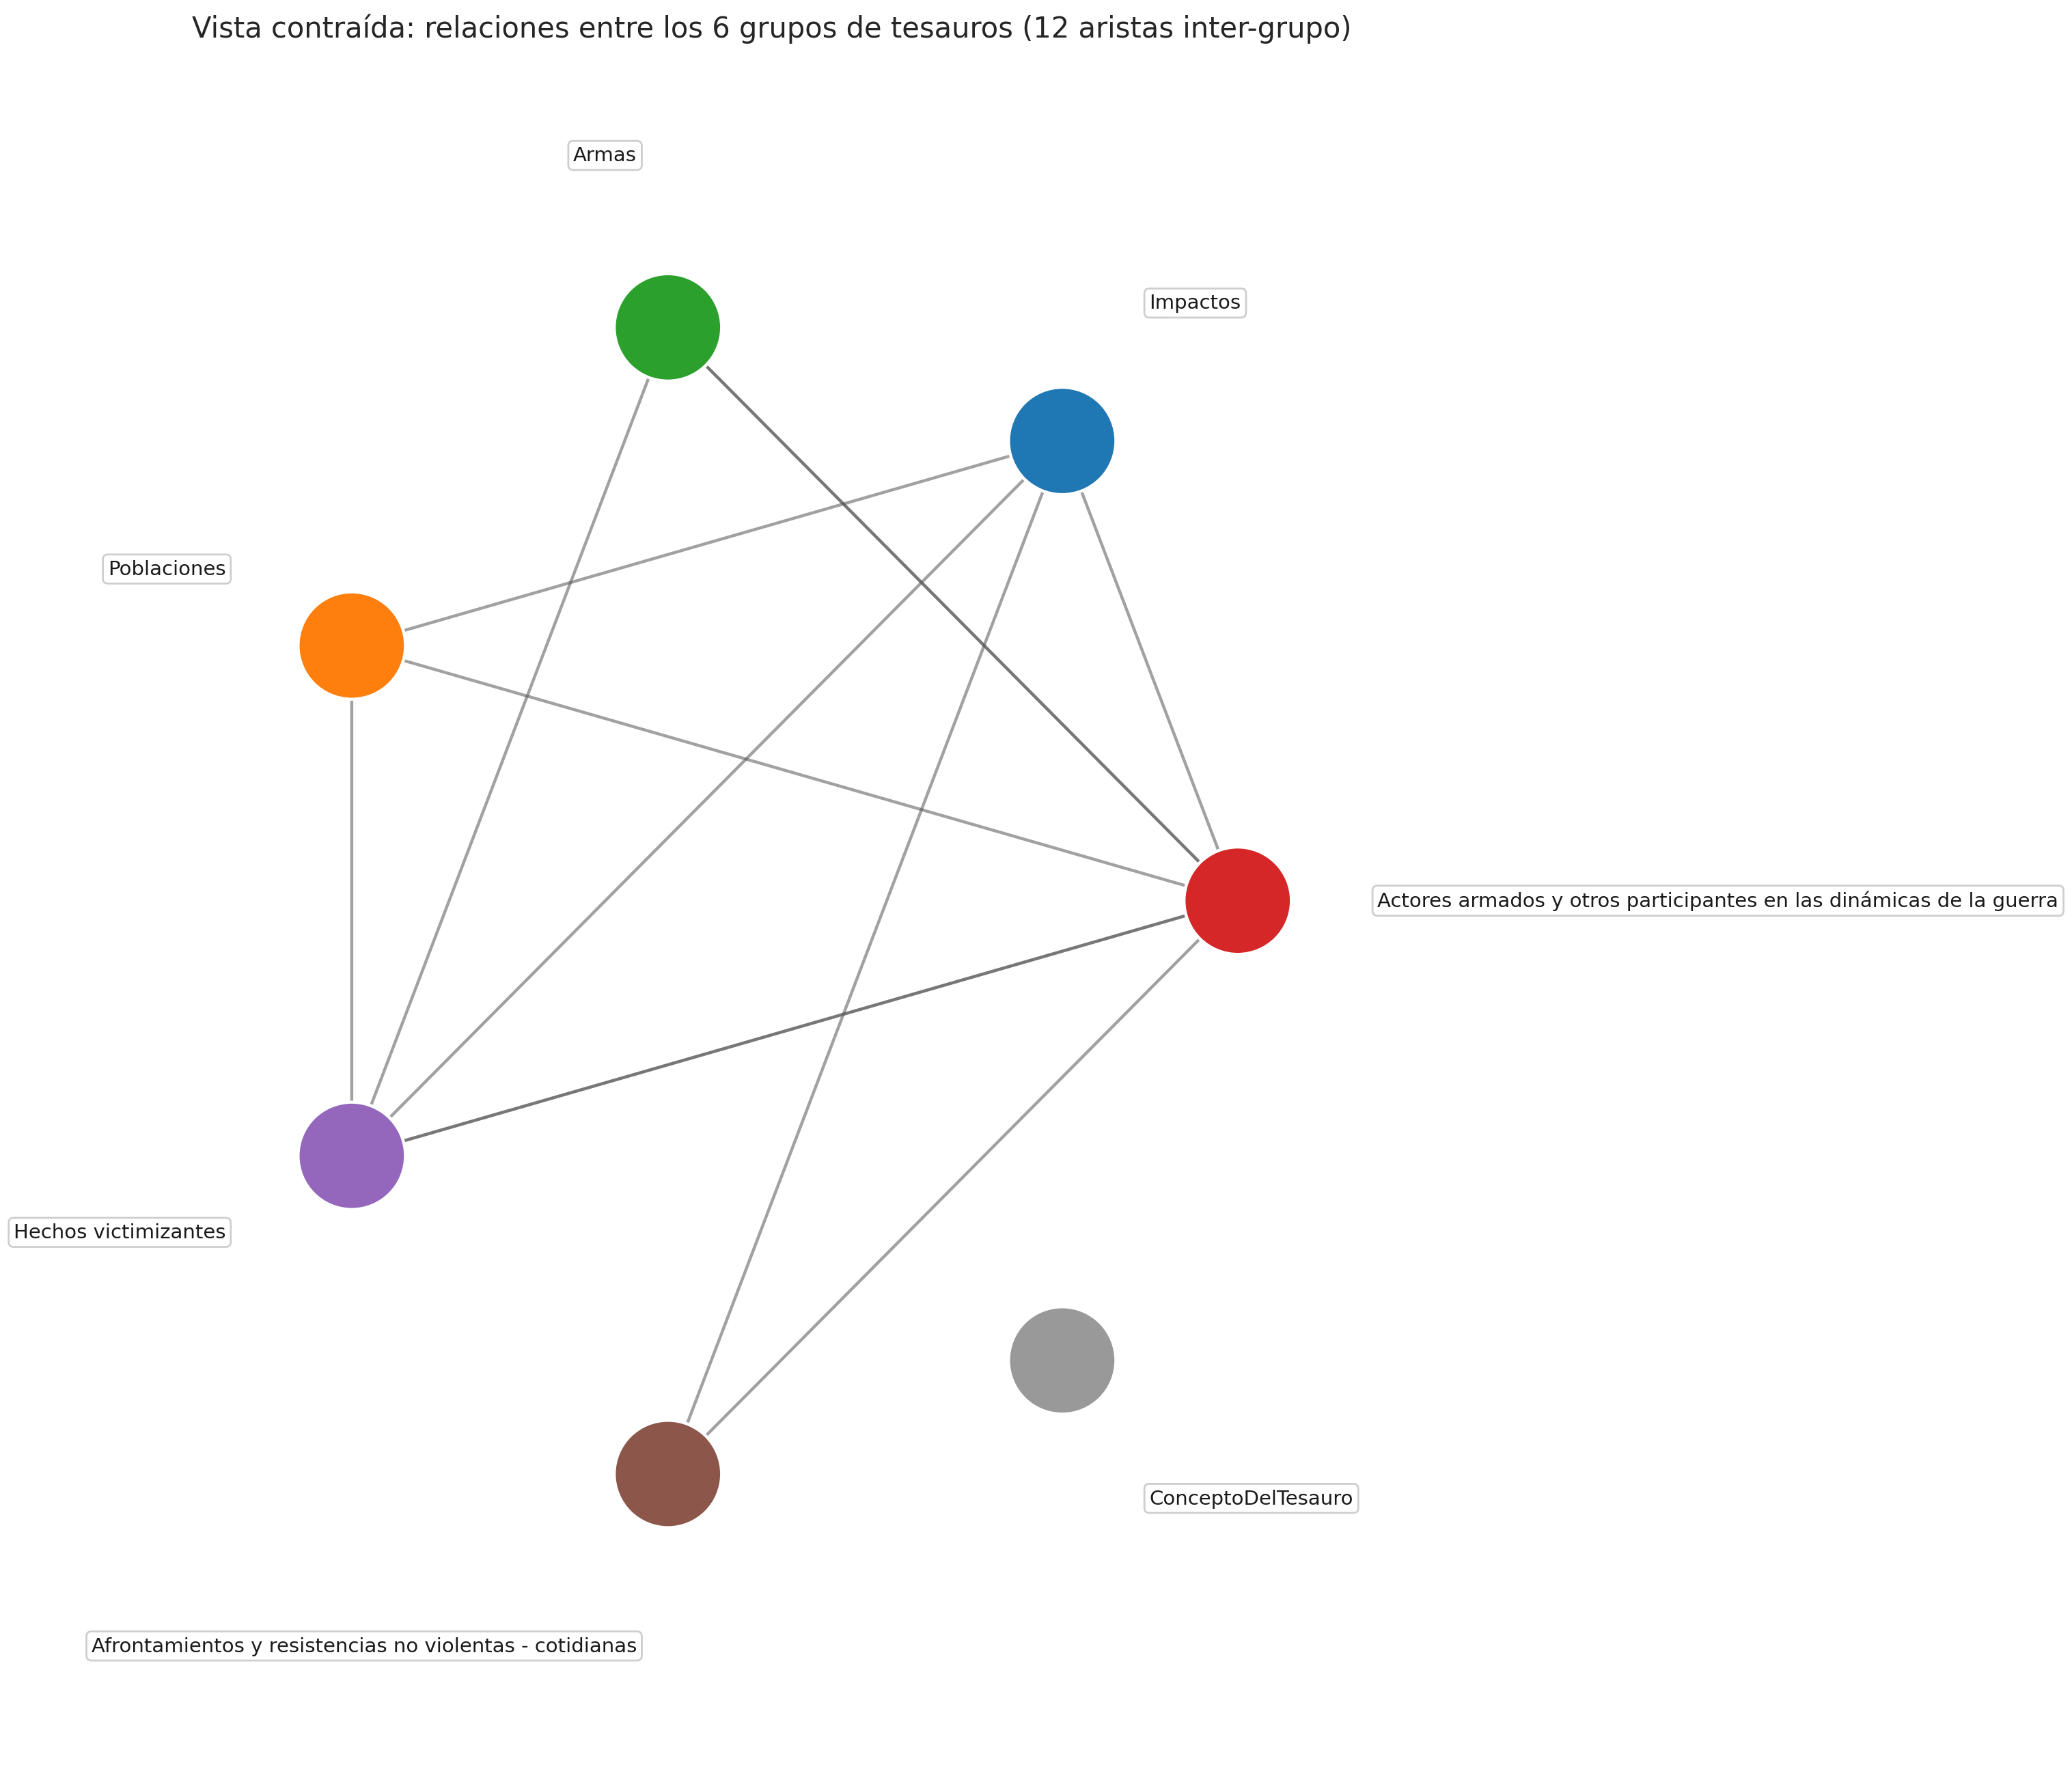
\includegraphics[width=0.62\textwidth]{figuras/grafo_ontologia_grupos.png}
    \caption{Vista contraída de la ontología: 6 grupos + superclase y las aristas inter-grupo del ciclo del conflicto (perpetradoPor, afectaA, generaImpacto, desarrollaAfrontamiento, respondeA, empleaArma).}
    \label{fig:ciclo}
\end{figure}

\subsection{Motor WordNet de relaciones semánticas}

Se implementó un motor que, dado un concepto de la ontología, consulta WordNet en español mediante \texttt{NLTK} y \texttt{omw-1.4} y devuelve las nueve relaciones del taller: sinonimia, antonimia, hiponimia, hiperonimia, meronimia, holonimia, troponimia, términos coordinados y derivación morfológica. El proceso incluye normalización del término (minúsculas, sin paréntesis), búsqueda de coincidencia exacta y, si falla, un fallback por segmentos con variantes ortográficas (singular/plural, sin acentos, guiones bajos, primer y último token de los compuestos). El código sigue un diseño orientado a objetos con patrones de diseño (Repository, Singleton, Abstract Factory, Strategy y Facade), de modo que añadir una relación exige solo registrar un nuevo extractor (principio Open/Closed).

\subsection{Consultas SPARQL}

Se diseñaron y ejecutaron \textbf{22 consultas SPARQL} contra la ontología con rdflib: 18 (tres por cada uno de los seis grupos) y 4 del modelo semántico (clases definidas con su fórmula, pares inversos del ciclo, la cadena completa Actor $\rightarrow$ Hecho $\rightarrow$ Población $\rightarrow$ Impacto $\rightarrow$ Afrontamiento e individuos por grupo). Cada consulta quedó documentada con su objetivo y su correspondencia con las relaciones TG/TE/TR del tesauro.


\section{Resultados}

\subsection{Estadísticas de la ontología}

La Tabla \ref{tab:ontologia} resume las estadísticas finales del artefacto OWL. La ontología es consistente (HermiT), se abre en Protégé y el razonador clasifica automáticamente las clases definidas: por ejemplo, \texttt{DesplazamientoForzado} es inferido subclase de \texttt{HechoPerpetradoPorActor} y las subclases de Poblaciones de \texttt{PoblacionConAfrontamiento}.

\begin{table}[H]
    \centering
    \caption{Estadísticas de la ontología OWL.}
    \small
    \setlength{\tabcolsep}{4pt}
    \begin{tabular}{l r}
    \hline
    Elemento & Valor \\
    \hline
    Clases & 623 (610 conceptos + 6 definidas + superclase) \\
    Individuos & 534 (términos hoja) \\
    Object properties & 17 (5 estructurales + 12 del ciclo en 6 pares inversos) \\
    Clases definidas & 6 (\texttt{owl:equivalentClass}) \\
    Axiomas TR (\texttt{relacionadoCon}) & 50 \\
    Axiomas \texttt{perpetradoPor}/\texttt{esVictimaDe} & 12 (heurística) + 1 (raíz) \\
    Axiomas del ciclo del conflicto & 7 (raíz) \\
    Triples & 9.812 \\
    Validación & rdflib, HermiT (consistente y clasifica), Protégé 5.6.9 \\
    \hline
    \end{tabular}
    \label{tab:ontologia}
\end{table}

\begin{figure}[htbp]
    \centering
    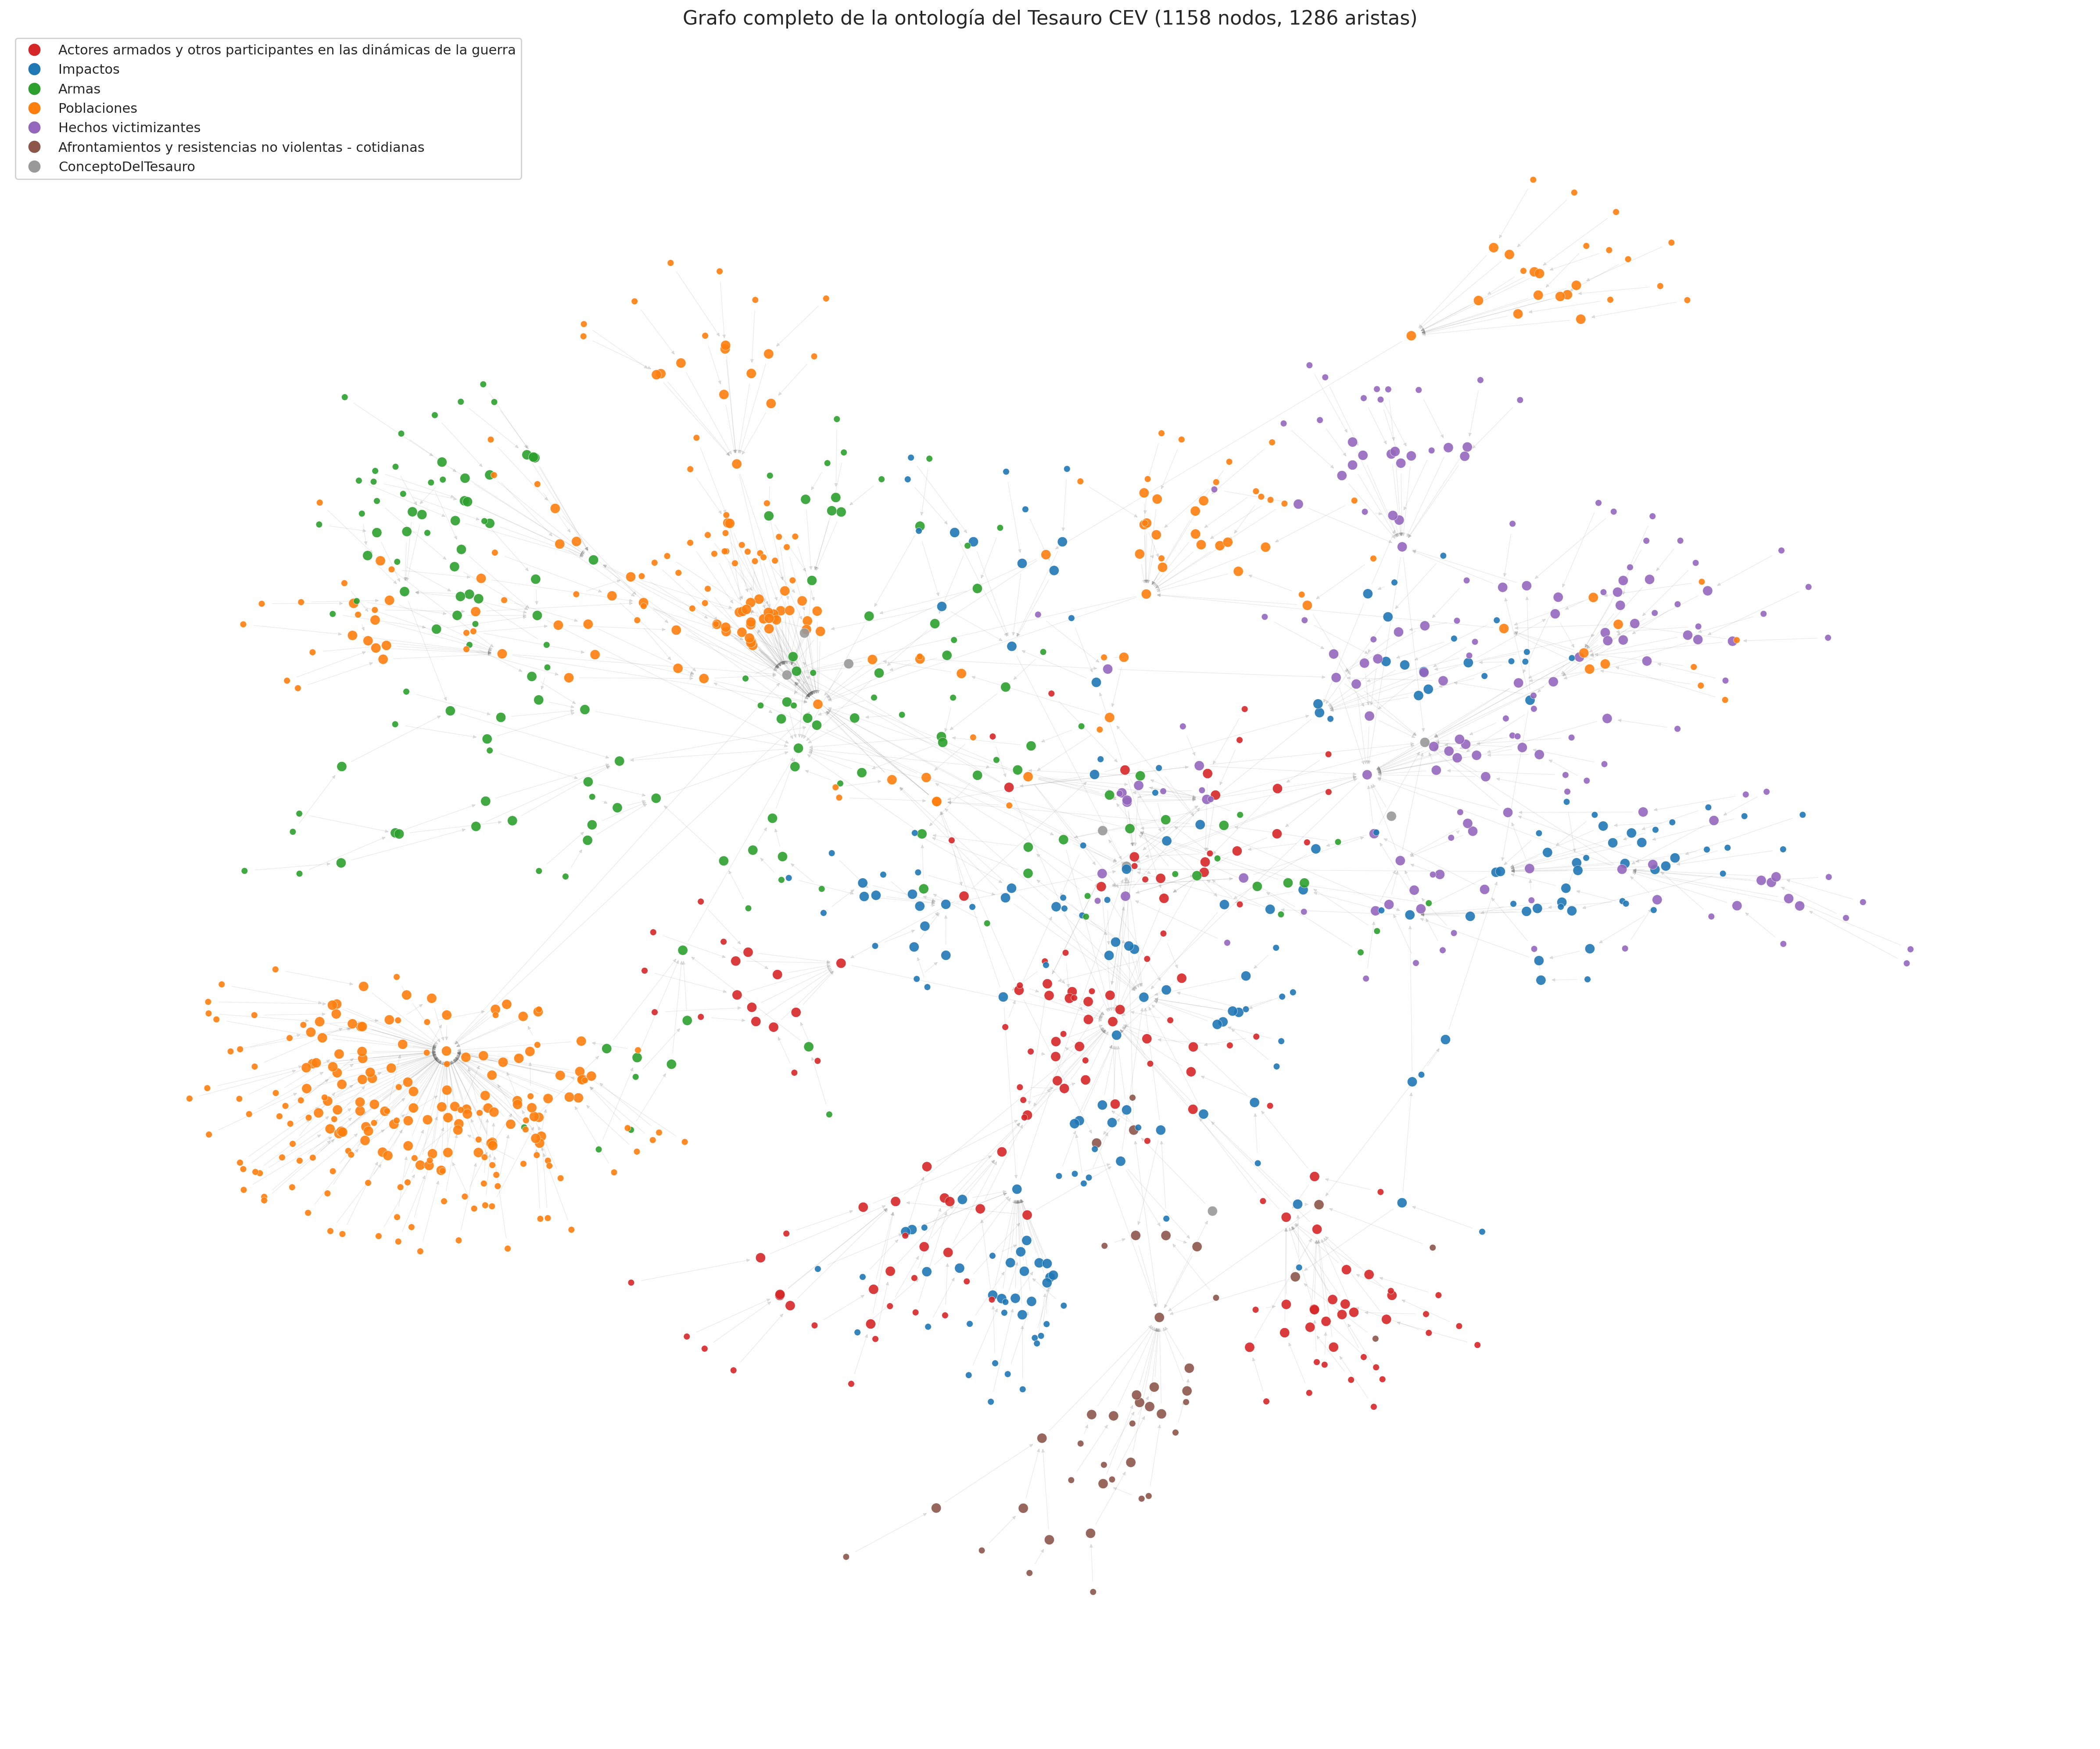
\includegraphics[width=0.85\textwidth]{figuras/grafo_ontologia_completo.png}
    \caption{Grafo completo de la ontología: 1.158 nodos y 1.286 aristas, clases e individuos coloreados por grupo raíz.}
    \label{fig:grafo}
\end{figure}

\subsection{Cobertura y relaciones de WordNet}

El análisis masivo cubrió \textbf{610 conceptos} de los seis grupos con una cobertura global del \textbf{50,5\,\%} (308 conceptos con al menos una relación). La cobertura varía fuertemente entre grupos: Hechos victimizantes 79,8\,\%, Afrontamientos 73,9\,\% (vía fallback de segmentos), Impactos 73,8\,\%, Actores armados 69,1\,\%, Armas 51,0\,\% y Poblaciones 16,8\,\% (vocabulario institucional ausente de WordNet general). La coincidencia exacta en omw-1.4 es baja (6,1\,\%); casi toda la cobertura se obtiene con el fallback por segmentos.

\begin{table}[H]
    \centering
    \caption{Relaciones semánticas extraídas por tipo (total 54.130).}
    \small
    \setlength{\tabcolsep}{4pt}
    \begin{tabular}{l r r}
    \hline
    Tipo de relación & Cantidad & \% del total \\
    \hline
    Coordinados & 24.920 & 46,0 \\
    Hiponimia & 22.290 & 41,2 \\
    Sinonimia & 2.638 & 4,9 \\
    Hiperonimia & 2.082 & 3,8 \\
    Derivación & 1.566 & 2,9 \\
    Meronimia & 310 & 0,6 \\
    Antonimia & 163 & 0,3 \\
    Holonimia & 80 & 0,1 \\
    Troponimia & 81 & 0,1 \\
    \hline
    \textbf{Total} & \textbf{54.130} & \textbf{100,0} \\
    \hline
    \end{tabular}
    \label{tab:relaciones}
\end{table}

Coordinados e hiponimia concentran el 87,2\,\% de las relaciones: son las relaciones ``más baratas'' de calcular y también las más ruidosas, pues los conceptos compuestos que no existen como lema se resuelven por núcleos polisémicos (vida, familia, género) cuyos múltiples synsets disparan decenas de hipónimos. Los 15 conceptos con más relaciones acumulan el 36,2\,\% del total, lo que confirma la ambigüedad del núcleo de fallback; la sinonimia, la hiperonimia y la derivación son cualitativamente más valiosas para expansión de consultas y desambiguación. La correlación entre profundidad jerárquica y número de relaciones es débil (Spearman $\rho = -0{,}180$): la especificidad del dominio, no la posición jerárquica, determina la cobertura.

\begin{figure}[htbp]
    \centering
    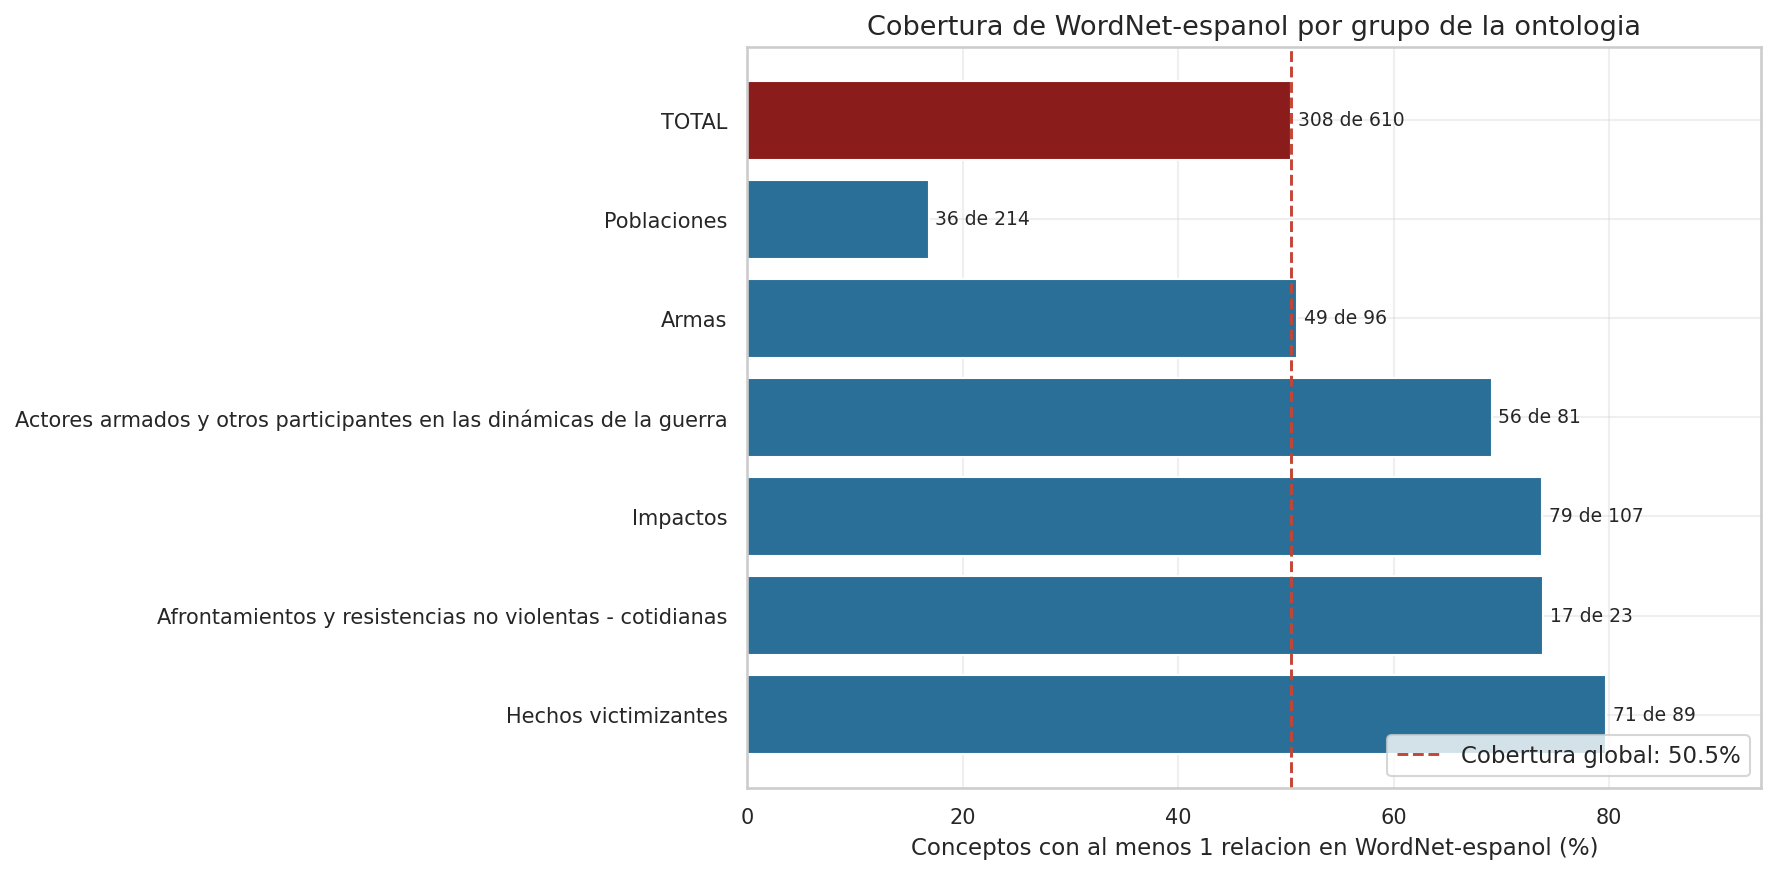
\includegraphics[width=0.8\textwidth]{figuras/cobertura_wordnet_conceptos.png}
    \caption{Cobertura de WordNet en español por grupo, ordenada de mayor a menor, con el total global.}
    \label{fig:cobertura}
\end{figure}

\begin{figure}[htbp]
    \centering
    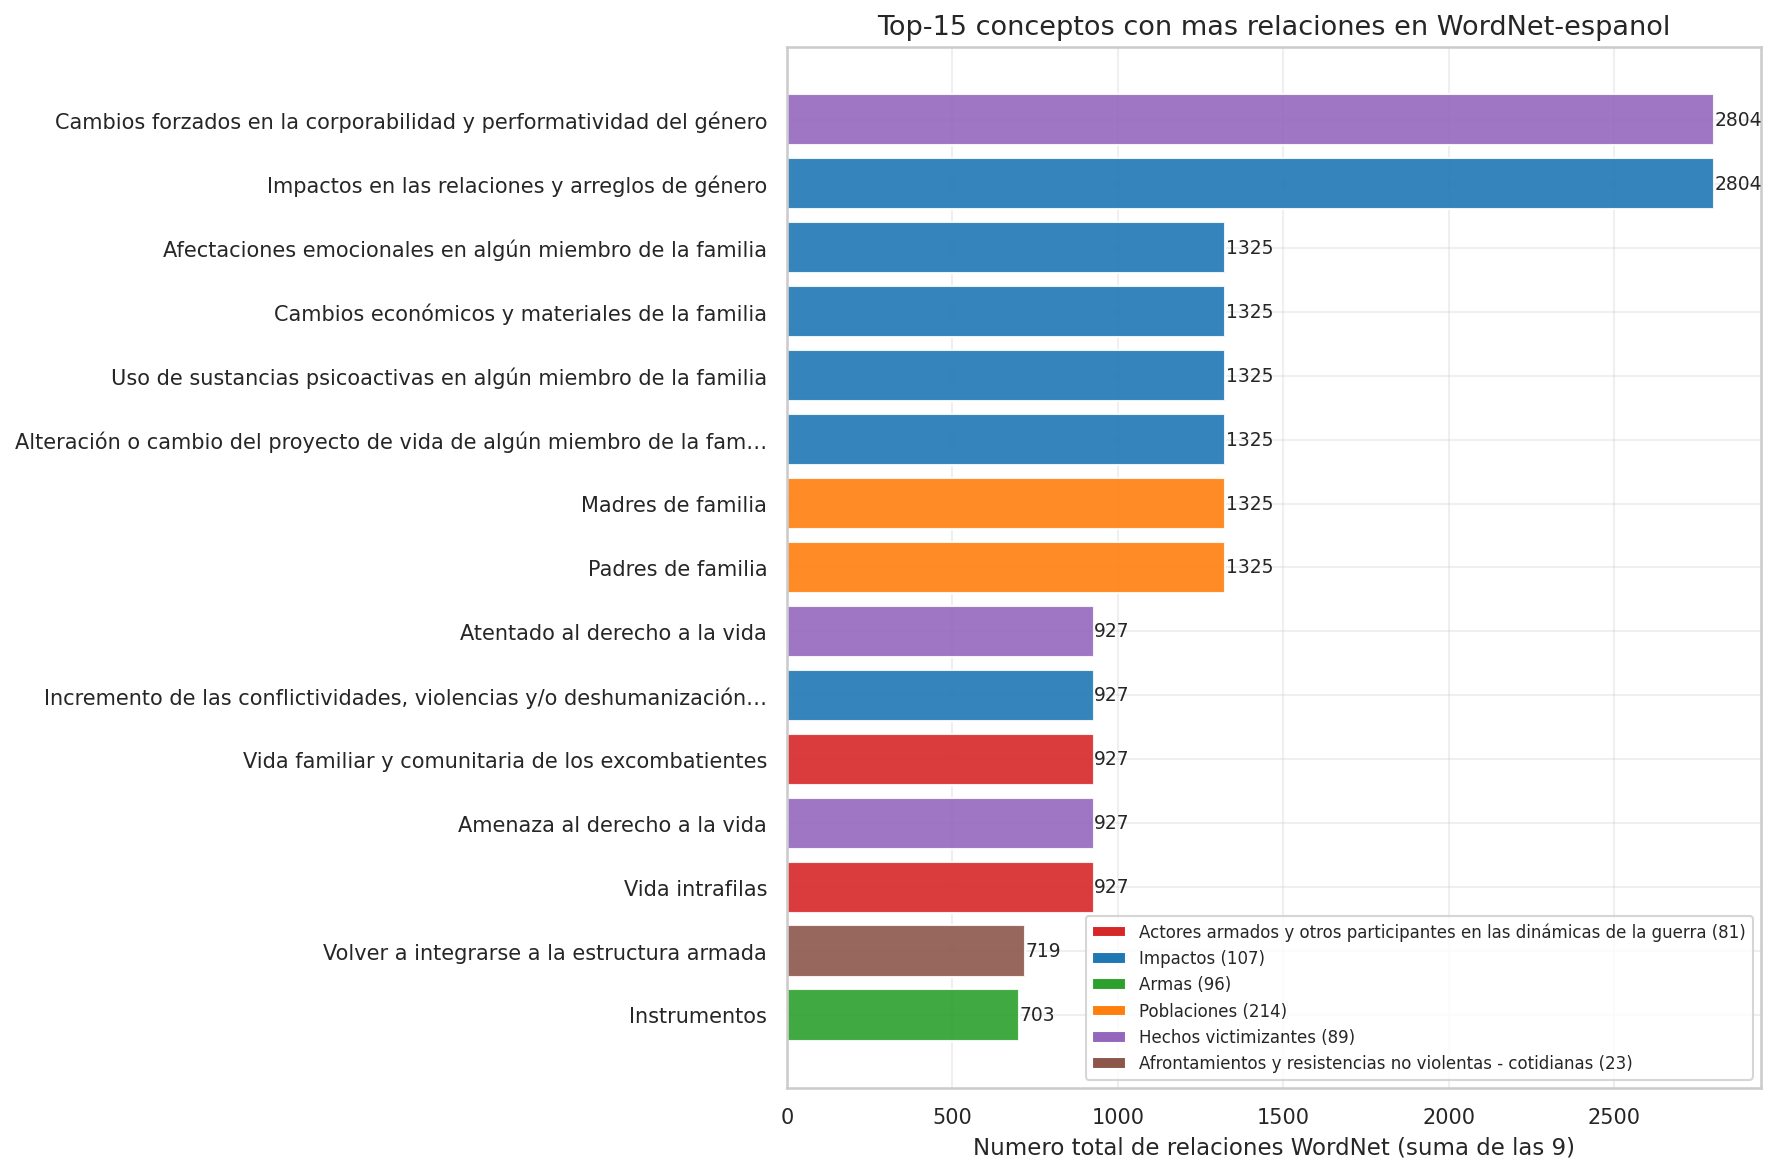
\includegraphics[width=0.8\textwidth]{figuras/top_relaciones_conceptos.png}
    \caption{Top-15 conceptos con más relaciones en WordNet: núcleos polisémicos que concentran el ruido del fallback.}
    \label{fig:top}
\end{figure}

\subsection{Consultas SPARQL}

Las 22 consultas se organizaron en tres patrones por grupo (estructura jerárquica TG/TE, individuos y población, y relaciones/cruces TR) más la sección del modelo semántico. Entre los resultados destacan: la jerarquía del grupo de Afrontamientos (23 filas), las clases definidas con su fórmula (6), los 7 axiomas del ciclo, los individuos por grupo (534 en total) y la consulta M.3, que recorre la cadena completa Actor $\rightarrow$ Hecho $\rightarrow$ Población $\rightarrow$ Impacto $\rightarrow$ Afrontamiento y devuelve el ciclo cerrado. Estas consultas se ejecutan en milisegundos con resultado determinista, algo que ningún método estadístico plano garantiza.


\section{Reflexión: ¿qué ventajas aporta representar conocimiento en ontologías frente a un análisis plano de texto en PLN?}

La pregunta del taller es el corazón de este trabajo, y los resultados permiten sostener cuatro argumentos.

\subsection{Semántica explícita y compartida}

El análisis plano de texto ---bolsas de palabras, n-gramas, frecuencias o incluso embeddings--- trata el lenguaje como una secuencia de símbolos cuyo significado queda implícito y depende del corpus. Una ontología declara explícitamente qué significa cada término: clases, individuos, propiedades, axiomas de inversa y de simetría. En este taller, el Tesauro CEV pasó de ser una lista de 12.341 cadenas a un artefacto en el que cada concepto tiene una identidad formal (IRI), un lugar en la jerarquía (\texttt{esParteDe}/\texttt{subClassOf}), su procedencia anotada (\texttt{cev:grupo}, \texttt{cev:eje}) y relaciones semánticas con otros conceptos. Este conocimiento es legible por humanos y por máquinas, y se publica en un estándar interoperable (OWL/RDF), algo que un análisis plano no puede ofrecer.

\subsection{Razonamiento e inferencia automática}

La ventaja más profunda es la posibilidad de \textbf{inferir conocimiento que no está escrito}. El razonador HermiT deriva automáticamente consecuencias de los axiomas: las propiedades inversas (\texttt{esParteDe}/\texttt{parteDe}, \texttt{afectaA}/\texttt{esAfectadaPor}) se razonan en ambas direcciones, la simetría de \texttt{relacionadoCon} se aplica sin declararla dos veces, y las clases definidas clasifican conceptos que nunca declararon su rol explícitamente. En este trabajo, \texttt{DesplazamientoForzado} fue inferido subclase de \texttt{HechoPerpetradoPorActor} y las subclases de Poblaciones de \texttt{PoblacionConAfrontamiento}: el razonador ``descubrió'' que toda población que desarrolla afrontamientos pertenece a la clase definida correspondiente. En un análisis plano, esa relación causal exigiría costosos pipelines de extracción de información, con resultados probabilísticos y no verificables. Las consultas SPARQL, por su parte, responden preguntas estructuradas ---¿qué actores perpetraron qué hechos? ¿qué impactos generaron? ¿qué afrontamientos desarrollaron las poblaciones?--- en milisegundos y con resultado determinista: la consulta del ciclo completo Actor $\rightarrow$ Hecho $\rightarrow$ Población $\rightarrow$ Impacto $\rightarrow$ Afrontamiento devuelve exactamente el camino causal modelado, sin ambigüedad.

\subsection{Reutilización y evolución}

La ontología es un activo incremental e interoperable: los 41 grupos del tesauro pueden incorporarse sin rediseñar el modelo, nuevos recursos léxicos pueden alimentar la extracción sin tocar el artefacto, y el OWL es portable entre herramientas (owlready2, rdflib, Protégé, HermiT). El diseño orientado a objetos del código refuerza esta propiedad: añadir una relación semántica exige registrar un nuevo extractor, no modificar el motor. Un análisis plano de texto, en cambio, es un resultado puntual atado a un corpus y a un pipeline específico, difícil de reutilizar y de auditar.

\subsection{Complementariedad, no sustitución}

Ambas aproximaciones se potencian: WordNet enriquece la ontología con sinonimia, hiponimia o antonimia que el tesauro no declara, mientras que la ontología delimita el dominio y protege al análisis plano de su principal debilidad, la polisemia. Al anclar los términos a clases formalizadas ---distinguir ``desplazamiento'' como hecho victimizante de ``desplazamiento'' como movimiento físico--- se reduce la ambigüedad que degrada los métodos estadísticos. El análisis plano sigue siendo insustituible a escala masiva y para conocimiento emergente no modelado; la ontología aporta precisión, trazabilidad y razonamiento donde el dominio está estructurado, como ocurre con el Tesauro CEV.

En síntesis, el taller demuestra que un tesauro de dominio puede transformarse en una ontología operable por razonadores y consultable formalmente, y que esta representación no compite con el PLN plano sino que lo complementa: fija el vocabulario, desambigua los términos y habilita inferencias que el texto, por sí solo, no puede responder.


\section{Conclusiones}

Se construyó una ontología OWL consistente de 623 clases y 534 individuos a partir de seis grupos del Tesauro CEV (609 términos), con un modelo semántico fuerte ---17 object properties (6 pares inversos del ciclo del conflicto), 7 axiomas raíz y 6 clases definidas que el razonador HermiT clasifica automáticamente---, enriquecida con 54.130 relaciones léxicas de WordNet en español (cobertura 50,5\,\% sobre 610 conceptos) y validada con HermiT y Protégé. Se ejecutaron 22 consultas SPARQL documentadas, incluida la consulta del ciclo completo del conflicto.

La cobertura parcial de WordNet (50,5\,\%) y la asimetría de las relaciones extraídas permiten calibrar el valor real de los recursos léxicos multilingües para dominios especializados: el fallback por segmentos conecta el vocabulario jerárquico del tesauro con WordNet, pero los núcleos polisémicos generan ruido en hiponimia y coordinados. El modelo semántico fuerte, por su parte, demuestra que la ontología no solo organiza términos sino que permite inferir y consultar ciclos causales, respondiendo a la pregunta central del taller: representar conocimiento en ontologías aporta semántica explícita, razonamiento automático, reutilización y complementariedad con el análisis plano de texto en PLN.


\nocite{*}
\bibliographystyle{apalike}
\newpage
\bibliography{references}

\end{document}
